\documentclass{oci}
\usepackage[utf8]{inputenc}
\usepackage{lipsum}
\usepackage{tikz}

\title{Problema Presidencial: Paltas Promedio}

\begin{document}
\begin{problemDescription}
En el último discurso presidencial, se explicó el incremento de la actividad
criminal a nivel país en base al reciente alza del precio de la palta Hass.
Esta correlación, que la presidencia denomina ICPC (Índice de Correlación entre
Paltas y Crimen) llegaría supuestamente al 65\%.
Ahora solo necesitan una forma de convencer a la población de que este índice 
completamente inventado es estadísticamente significativo.
Para ello, la Presidencia de la República solicitó a la Organización de
Coincidencias Intencionales, también conocida como OCI, encontrar la mayor
muestra de datos posible que valide esta estadística.

Dentro de los datos que la OCI tiene a disposición, posee un arreglo con los
valores diarios del ICPC en los últimos $N$ días, y la misión es encontrar el
período más largo de días consecutivos en que el promedio del ICPC alcanza un
valor deseado $T$.

Por ejemplo, considere el siguiente arreglo con los valores del ICPC en los
últimos 7 días:
\begin{center}
  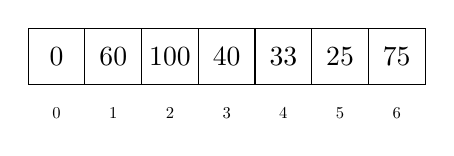
\begin{tikzpicture}[scale = 0.6]
    \foreach \i in {0,...,6}{
      \draw (\i*1.2,0) rectangle +(1.2,1.2);
      \node at (\i*1.2+0.6,-0.6) {\scalebox{0.6}{$\i$}};
    }
    \node at (0*1.2+0.6,0.6) {$0$};
    \node at (1*1.2+0.6,0.6) {$60$};
    \node at (2*1.2+0.6,0.6) {$100$};
    \node at (3*1.2+0.6,0.6) {$40$};
    \node at (4*1.2+0.6,0.6) {$33$};
    \node at (5*1.2+0.6,0.6) {$25$};
    \node at (6*1.2+0.6,0.6) {$75$};
  \end{tikzpicture}
\end{center}

Si se desea mostrar a la gente que el ICPC es de $T=50\%$, tanto el periodo
comprendido entre las posiciones 0 y 3 como el comprendido entre las posiciones
5 y 6 tienen un promedio exactamente 50\%.
Como el periodo entre las posiciones 0 y 3 es más largo, la OCI prefiere
reportar este.

La OCI ha descubierto que participas de las olimpiadas de informática y por lo mismo
piensa que eres la persona perfecta para ayudarlos en su nuevo plan de
manipulación social.
\end{problemDescription}

\begin{inputDescription}
  La primera línea de la entrada contiene dos enteros $N$ y $T$ separados por
  un espacio.

  La siguiente línea contiene $N$ enteros $A_i$ separados por espacios,
  describiendo el arreglo $A$ de valores del ICPC en los últimos $N$
  días.

  Puedes asumir que las siguientes restricciones siempre se cumplen:

  \begin{itemize}
  \item $1 \le N \le 10^6$

  \item $0 \le T \le 100$

  \item $0 \le A_i \le 100$
  \end{itemize}
\end{inputDescription}

\begin{outputDescription}
La salida debe contener una única línea con dos enteros $S$ y $L$ separados por
un espacio.
Estos enteros deben describir el período de días consecutivos que se le mostrará
a la población, es decir, el subarreglo más largo de $A$ cuyo promedio es
exactamente el valor $T$.

Específicamente, $S$ debe ser la posición dentro de $A$ donde comienza el
subarreglo y $L$ debe ser su largo.
El índice $0$ corresponde al primer elemento.
 
Si hay dos o más subarreglos del mismo largo que cumplen con los requisitos, se
debe reportar el que comience primero (menor $S$).

Si no hay ningún subarreglo que cumpla con los requisitos, se debe imprimir
\texttt{-1}.
\end{outputDescription}

\begin{scoreDescription}
  \subtask{10}
  Se probarán varios casos donde $N \le 250$.
 
  \subtask{20}
  Se probarán varios casos donde $N \le 5000$.
 
  \subtask{40}
  Se probarán varios casos donde $N \le 10^6$ y además el arreglo $A$ estará ordenado de
  menor a mayor, es decir, $A_i \le A_{i+1}$ para todo $i$.
 
  \subtask{30}
  Se probarán varios casos donde $N \le 10^6$ y el arreglo $A$ no estará
  necesariamente ordenado.
\end{scoreDescription}

\begin{sampleDescription}
\sampleIO{sample-1}
\sampleIO{sample-2}
\sampleIO{sample-3}
\end{sampleDescription}

\end{document}
